\documentclass[12pt,a4paper,oneside,ngerman]{article}
\usepackage[utf8]{inputenc}
\usepackage{color}
\usepackage{tikz}
\usepackage{amsmath}
\usepackage{amssymb}
\usepackage{calc}
\usepackage{float}

\title{EZS}
\author{Simon Krücken}

\begin{document}
    
\begin{titlepage}
%    \maketitle
\end{titlepage}
\tableofcontents

\section{Unterlagenfreier Teil}

1. Definieren Sie den Begriff Realzeitsystem\\
Ein Realzeitsystem muss neben den funktionalen Anforderungen auch noch zeitliche Anforderungen genügen.\\

2. Wie lauten die Beiden Realzeitbedingungen (genaue Angabe)?\\

\begin{itemize}
	\item 1. Realzeitbedingung:\\ \(\rho_{max,ges} = \displaystyle\sum_{j=1}^n \dfrac{t_{Emax,i}}{t_{Pin,i}} \leq c\) mit c = Anzahl Rechnerkerne
	\item 2. Realzeitbedingung: Für alle Rechenzeitanforderungen i muss gelten:\\ \( t_{Dmin,j} \leq t_{Rmin,j} \leq t_{Rmax,j} \leq t_{Dmax,j} \)
\end{itemize}

3. Erläutern Sie anhand der Nutzen-Funktion mithilfe einer genauen Skizze den Unterschied zwischen harter und weicher Realzeit!\\
\begin{figure}[H]
	\centering
	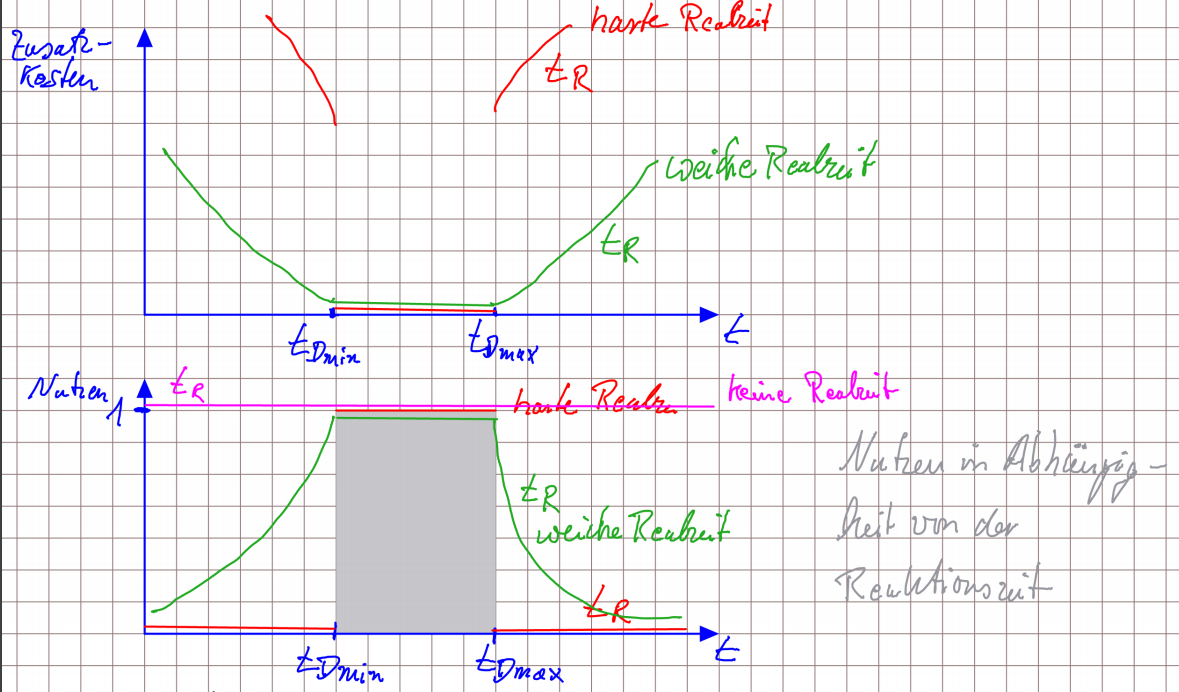
\includegraphics[scale=0.3]{umlet/harte_weiche_realzeit.png}
\end{figure}

\section[Formeln]{Formeln}

\(t_{Pmin,i} = minimal\) =$>$ \(t_{max,i} = \dfrac{1}{ t_{Pmin,i} }\) \\
\(t_{Pmax,i} = maximal\) \textcolor{gray}{$<$= uninteressant} \\
\(t_{Dmin,i}\) = minimal zulässige Reaktionszeit \\
\(t_{Dmax,i}\) = maximal zulässige Reaktionszeit

\begin{description}
    \item - Ausführuntgszeit (Executiontime) = Rechenzeit für eine RZ-Anforderung (ohne Warte oder Schlafzeiten)	
        \begin{description}
            \item - WCET \(t_{Emax,i}\) --$>$ Erfahrung oder Messen \textcolor{gray}{Worstcase}
            \item - BCET \(t_{Emin,i}\) = 0 \textcolor{gray}{Bestcase}
        \end{description}
    \end{description}

\(T_{Rmax,i}\) = maximale Reaktionszeit \\
\(T_{Rmin,i}\) = minimale Reaktionszeit \\
\(T_{R,i}\) = \textcolor{red}{\(t_{W,i}\)} \(+ t_{E,i}\) wobei \textcolor{red}{ \(t_{W,i}\) } Summe aller Wartezeiten

- Latenzzeit \(t_{L_i}\)
\textcolor{blue}{
	- Interrup Latenzzeit
	- Tasklatenzzeit
}

\(\rho_i = \dfrac{t_{E,i}}{t_{P,i}}\) Auslastung dur RZ-Anforderung i

\(\rho_{max,i} = \dfrac{t_{Emax,i}}{t_{Pin,i}}\) Worstcase, max. Auslastung

\fbox{
	\parbox{\textwidth}
	{
		1. RT Bedingung

		\(\rho_{max,ges} = \displaystyle\sum_{j=1}^n \dfrac{t_{Emax,i}}{t_{Pin,i}} \leq c\) \\
		j = für alle RZ-Anforderungen,
		c = Anzahl der Rechnerkerne
	}
}

\fbox{
	\parbox{\textwidth}
	{	
		\emph{Technischer prozess: }\\
		\begin{description}
			\item - \textcolor{blue}{\(t_{P,i}\)} = Prozesszeit, zeitlicher Abstand zwischen zwei RT-Anforderungen \textcolor{blue}{i} \fbox{ \textcolor{blue}{\(t_{Pmin,i}\)}}
			\item - \textcolor{blue}{\(t_{Dmin,i}\)} = minimal zulässige Reaktionszeit
			\item - \textcolor{blue}{\(t_{Dmax,i}\)} = maximal zulässige Reaktionszeit
			\item - \textcolor{blue}{\(t_{Ph,i}\)} = Phase, zeitlicher Abstand zwischen zwei \textcolor{red}{unterschiedlicher} Ereignise
		\end{description}
	}
}

\fbox{
	\parbox{\textwidth}
	{	
		\emph{Rechenprozesse: }\\
		\begin{description}
			\item - \textcolor{blue}{\(t_{Emin,i}\)} = minimale Ausführungszeit BCET
			\item - \textcolor{blue}{\(t_{Emax,i}\)} = maximale Ausführungszeit WCET
			\item - \textcolor{blue}{\(t_{Rmin,i}\)} = minimale Reaktionszeit
			\item - \textcolor{blue}{\(t_{Rmax,i}\)} = maximale Reaktionszeit\\ \rotatebox[origin=c]{180}{$\Lsh$} Zeitlicher Abstand zwischen dem Eintreffen einer RT-Anforderung \textcolor{blue}{i} und dem Ende der Bearbeitung
			\item - \textcolor{blue}{\(t_{W,i}\)} = Wartezeit, Summe der Zeiten, in der eine Codesequenz arbeiten könnte, aber nicht dran kommt.
		\end{description}
	}
}

\fbox{
	\parbox{\textwidth}
	{	
		\emph{Systemsoftware: }\\
		\begin{description}
			\item - \textcolor{blue}{\(t_{L,i}\)} = Latenzzeit, zeitlicher Abstand zwischen dem Eintreffen einer RT-Anforderung \textcolor{blue}{i} und dedm Start der Bearbeitung
			\item - \textcolor{blue}{Schedulingverfahren}
		\end{description}
	}
}

\fbox{
	\parbox{\textwidth}
	{
		1. RT Bedingung

		\(\rho_{max,ges} = \displaystyle\sum_{j=1}^n \dfrac{t_{Emax,j}}{t_{Pmin,j}} \leq c\) \\
		j = für alle RZ-Anforderungen,
		c = Anzahl der Rechnerkerne
	}
}

\fbox{
	\parbox{\textwidth}
	{
		2. RT Bedingung

		Für alle RZ-Anforderungen j muss gelten:

		\( t_{Dmin,j} \leq t_{Rmin,j} \leq t_{Rmax,j} \leq t_{Dmax,j} \)
	}
}

\fbox{
	\parbox{\textwidth}
	{
		Utilization
		\(u = \displaystyle\sum_{j=1}^n \dfrac{t_{Emax,j}}{ min(t_{Dmax,j}, t_{Pmin,j})} \)
	}
}

\end{document}